\documentclass[9pt]{beamer}
\usepackage[english]{babel}
\usepackage[utf8]{inputenc}
\usepackage{xcolor}
\definecolor{btublack}{cmyk}{0.1,0,0,0.8} 
\definecolor{btured}{cmyk}{0,1,0.9,0} 
\definecolor{fak1Color}{cmyk}{0.10,1.00,0,0} % magenta
\definecolor{fak2Color}{cmyk}{1,0.70,0,0}    % dark blue
\definecolor{fak3Color}{cmyk}{1,0,0.10,0}    % light blue
\definecolor{fak4Color}{cmyk}{0.45,0,1,0}    % light green
\usepackage{amsmath,amsfonts,amssymb}	
\usepackage{listings}
\usepackage{tikz}
\beamertemplatenavigationsymbolsempty	%Navigationsleiste ausblenden
\usetheme{btu} 
\usecolortheme{fak1} 
\usefonttheme{professionalfonts}
\usepackage{mathptmx}
\usepackage{helvet} 
%\usepackage{courier}
% \usepackage{avant} 
% \usepackage{chancery} 
% \usepackage{newcent} 
% \usepackage{palatino} 
%\usepackage{btulogo} 
%\titlegraphic{\BTUKeyVisualLeft}  
\titlegraphic{\hspace{0.45cm}
\includegraphics[scale=0.3]{mythos-logo}}
% small logo (visible on all other pages) 
\usepackage{btulogo} 
\newsavebox{\mybtulogo} 
\savebox{\mybtulogo}{\BTULogoStandardEnScale{BTUallgemein}{0.67}} 
\logo{\usebox{\mybtulogo}}
% mythos logo
\newsavebox{\mylogo} 
\savebox{\mylogo}{
\includegraphics[width=1.5cm]{mythos-logo}} 
%\logo{\usebox{\mylogo}}


% ========================================================================================
% PRESENTATION SETTINGS
% ========================================================================================
\author{\textbf{Robert Kuban}, Randolf Rotta}
\title{Base Architecture 2.0}
\subtitle{OS Reengineering for Parallelism}
%\institute{FG Verteilte Systeme/Betriebssysteme}
%\date[\today]{\today}
%\date{15. März 2016}
% title of table of contents pages
\newcommand{\outlineTitle}{Outline}
% title of bib slide
% \newcommand{\bibtitle}{Bibliography}

% show table of contents at the beginning of new sections
% \AtBeginSection[]{%
%     \frame{%
%         \frametitle{\outlineTitle}% title of the frame as defined above
%         % plain table of contents:
%         % \tableofcontents% 
%         % higlight current section and subsection:
%         \tableofcontents[currentsection]%
%         %\tableofcontents[currentsection,currentsubsection] % higlight current section and subsection
%         % highlight but do not show any subsections:
%         % \tableofcontents[currentsection, hideallsubsections]% 
%         % highlight and show only subsections of the current section:
%         % \tableofcontents[currentsection, hideothersubsections]%
%     }%
% }

\begin{document}

\frame[plain]{
  \titlepage
}

\logo{\usebox{\mylogo}}

\begin{frame}
  \frametitle{Outline}
  \tableofcontents%[currentsection]
\end{frame}

\section{Applications and Objectives}

\begin{frame}
  \frametitle{Target: Many-Core Processors}
  \framesubtitle{E.g. Intel XeonPhi Knights Corner}

  \begin{center}
    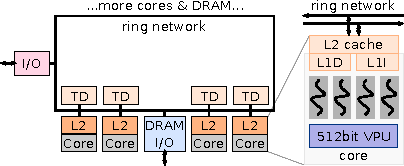
\includegraphics[height=3cm]{figures/hw-xeonphi}
  \end{center}
  %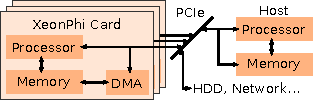
\includegraphics[height=2cm]{figures/hw-xeonphi-host}
  %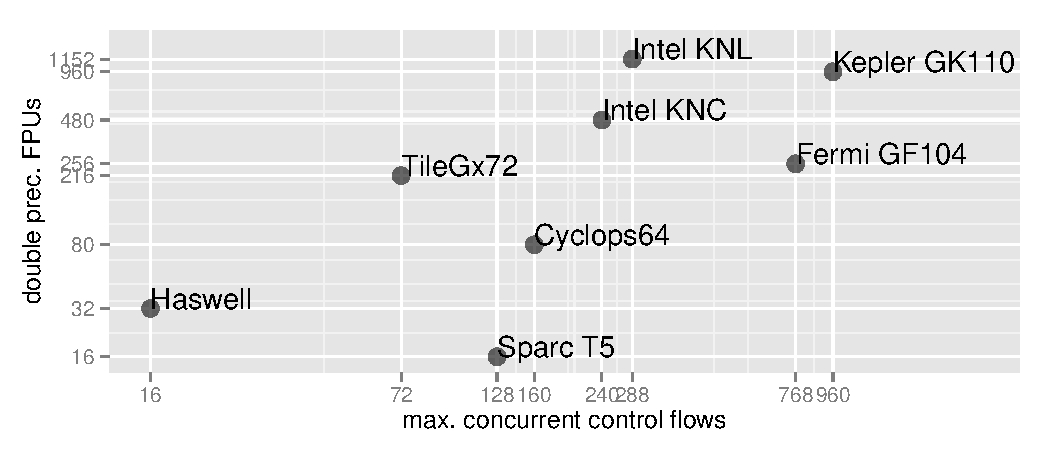
\includegraphics[height=5cm]{figures/manycore}

  \begin{itemize}
  \item optimised for max. parallel FP throughput in fixed power \& space budget 
  \item energy and area efficiency instead of single-thread performance
  \item ``heterogeneous'': shared memory but \alert{distributed behaviour} 
  \item[$\Rightarrow$] peak throughput \alert{requires parallelism on all layers}
  \end{itemize}
\end{frame}

\begin{frame}
  \frametitle{Many Threads on Many Cores}
  \framesubtitle{Functional requirements}

% TODO: replace block by figure. task/data flow graph nodes and threads; enclaves, supervisor 
\begin{block}{Application Scenarios}
\begin{itemize}
\item \alert{Dynamic HPC}: self-managed, shared resources
\item \alert{Compute Cloud}: 3rd-party tasks in supervised enclaves
\end{itemize}
\end{block}

\begin{block}{Implications}
\begin{itemize}
\item creating, placing, scheduling threads: \texttt{spawn}, \texttt{suspend}\ldots
\item sleeping, asynchronous \& preemptive notifications: \texttt{wait}, \texttt{notify}\ldots
\item manage physical memory \& logical addresses: \texttt{mmap}, \texttt{mprotect}\ldots
\item supervisor manages application threads:\\
  granting and revoking rights on \emph{supervised threads} -- not users
\end{itemize}
\end{block}
\end{frame}

\begin{frame}
  \frametitle{Scalable Throughput on Many Cores }
  \framesubtitle{Non-functional objectives}

  \begin{block}{Utilise many cores:}
    \begin{itemize}
    \item eliminate bottlenecks from hidden sharing % sharing is user's decision 
    \item move bookkeeping out of time-critical path % object deletion and cleanup
    \item \ldots offload to idle or dedicated cores % 
    \end{itemize}
  \end{block}

  \begin{block}{Utilise waiting time:}
    \begin{itemize}
    \item either sleep or work % no spin locks, no busy waiting
    \item non-blocking synchronisation, async.\ communication
    % \item bookkeeping tasks for idle time
    \end{itemize}
  \end{block}

  \begin{block}{Reduce overhead:}
    \begin{itemize}
    \item exploit locally shared hardware % local sharing of objects
    \item eliminate \& simplify OS policies % no on-demand allocation, no swapping, no demand paging, no fair time sharing
    \item optimise for small tasks \& messages % messages for control flow, shared memory for data
    \end{itemize}
  \end{block}
\end{frame}

\section{Lessons Learned}

\begin{frame}
  \frametitle{Outline}
  \tableofcontents[currentsection]
\end{frame}

% TODO more slides on the general topic, compare locks, wait-free, RCU, message passing
\begin{frame}
  \frametitle{Asynchronous Programming Model}
  
  \begin{block}{Current state: focus on tasks and placement}
    \begin{itemize}
    \item caller creates active message, sends to target core
    \item non-blocking execution via shared queues
    \item control flow by chaining of continuation tasks
    \end{itemize}
  \end{block}

  \vfill
  \begin{center}
    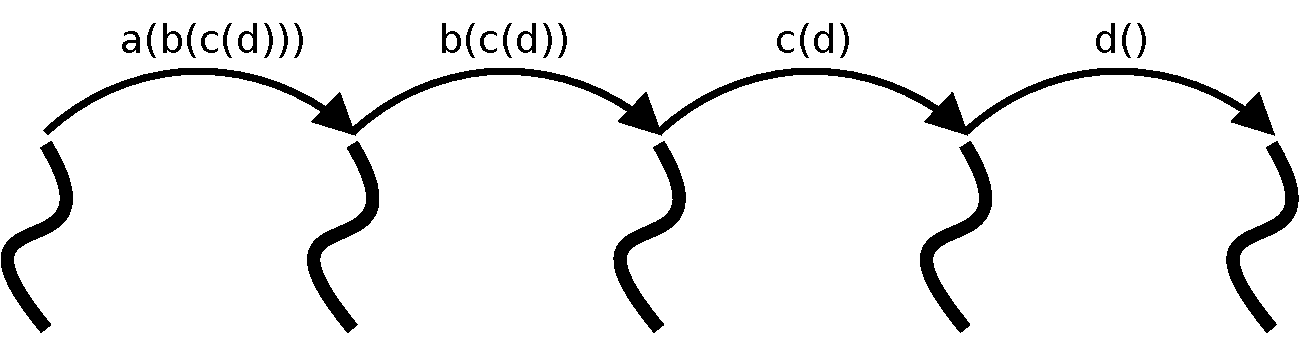
\includegraphics[height=2cm]{figures/continuations.pdf}
  \end{center}
  \vfill

  \begin{block}{Issues: low productivity, high error rate}
    \begin{itemize}
    \item caller responsible for synchronisation and placement
%    \item logic should not care about placement
    \item no flow control $\Rightarrow$ on-demand allocation, complex scheduling
    \end{itemize}
  \end{block}
\end{frame}
  
\begin{frame}
  \frametitle{Asynchronous Programming Model}

  \vfill
  \begin{center}
  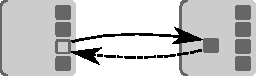
\includegraphics[height=2cm]{figures/asyncobj.pdf}
  \end{center}
  \vfill

  \begin{block}{Insight: deferred synchronous cycles}
    \begin{itemize}
    \item communicate between objects -- not cores
    \item target responsible for synchronisation and scheduling
    \item static allocation of task buffers
    \item inherent flow control
    \end{itemize}
  \end{block}
\end{frame}

\begin{frame}
  \frametitle{Kernel's Resource Management}

  \begin{block}{Current state: shared pools and reference counting}
    \begin{itemize}
    \item kernel owns all physical memory, core-local allocators
    \item smart pointers with reference counting
    \end{itemize}
  \end{block}

  \vfill
  \centering{
    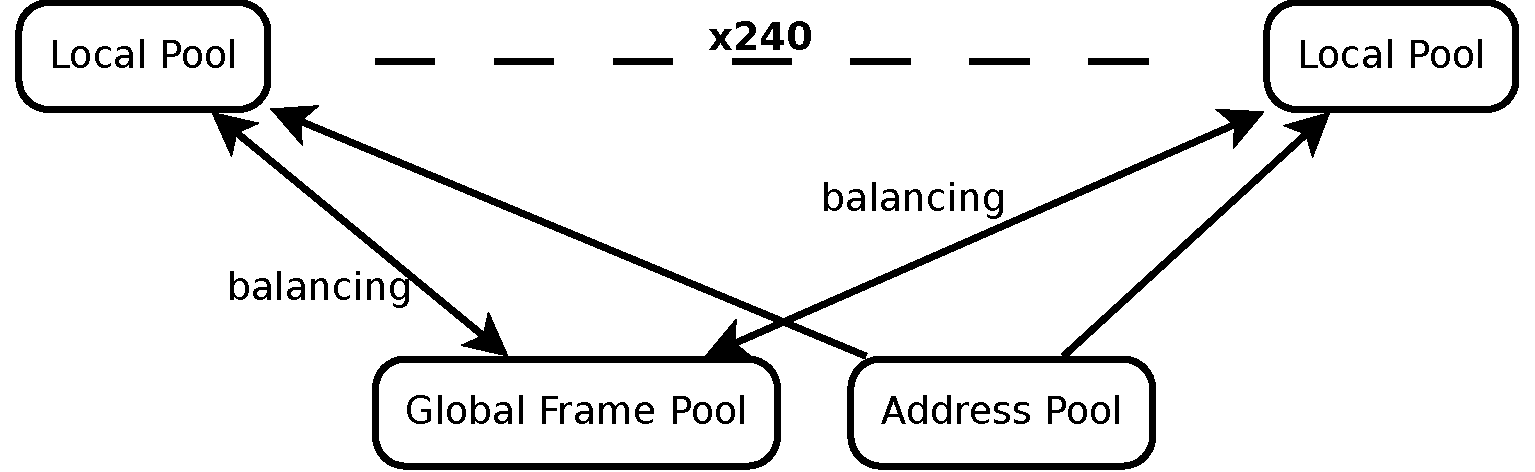
\includegraphics[height=3cm]{figures/mem-balancing.pdf}
  }
  \vfill
  
  \begin{block}{Issues: hidden sharing, complex, unreliable}
    \begin{itemize}
    \item implicit on-demand allocation \& balancing between pools
    \item cyclic references prevent cleanup; in-flight references ignored
    \end{itemize}
  \end{block}
\end{frame}

\begin{frame}
  \frametitle{Kernel's Resource Management}

  \vfill
  \begin{center}
  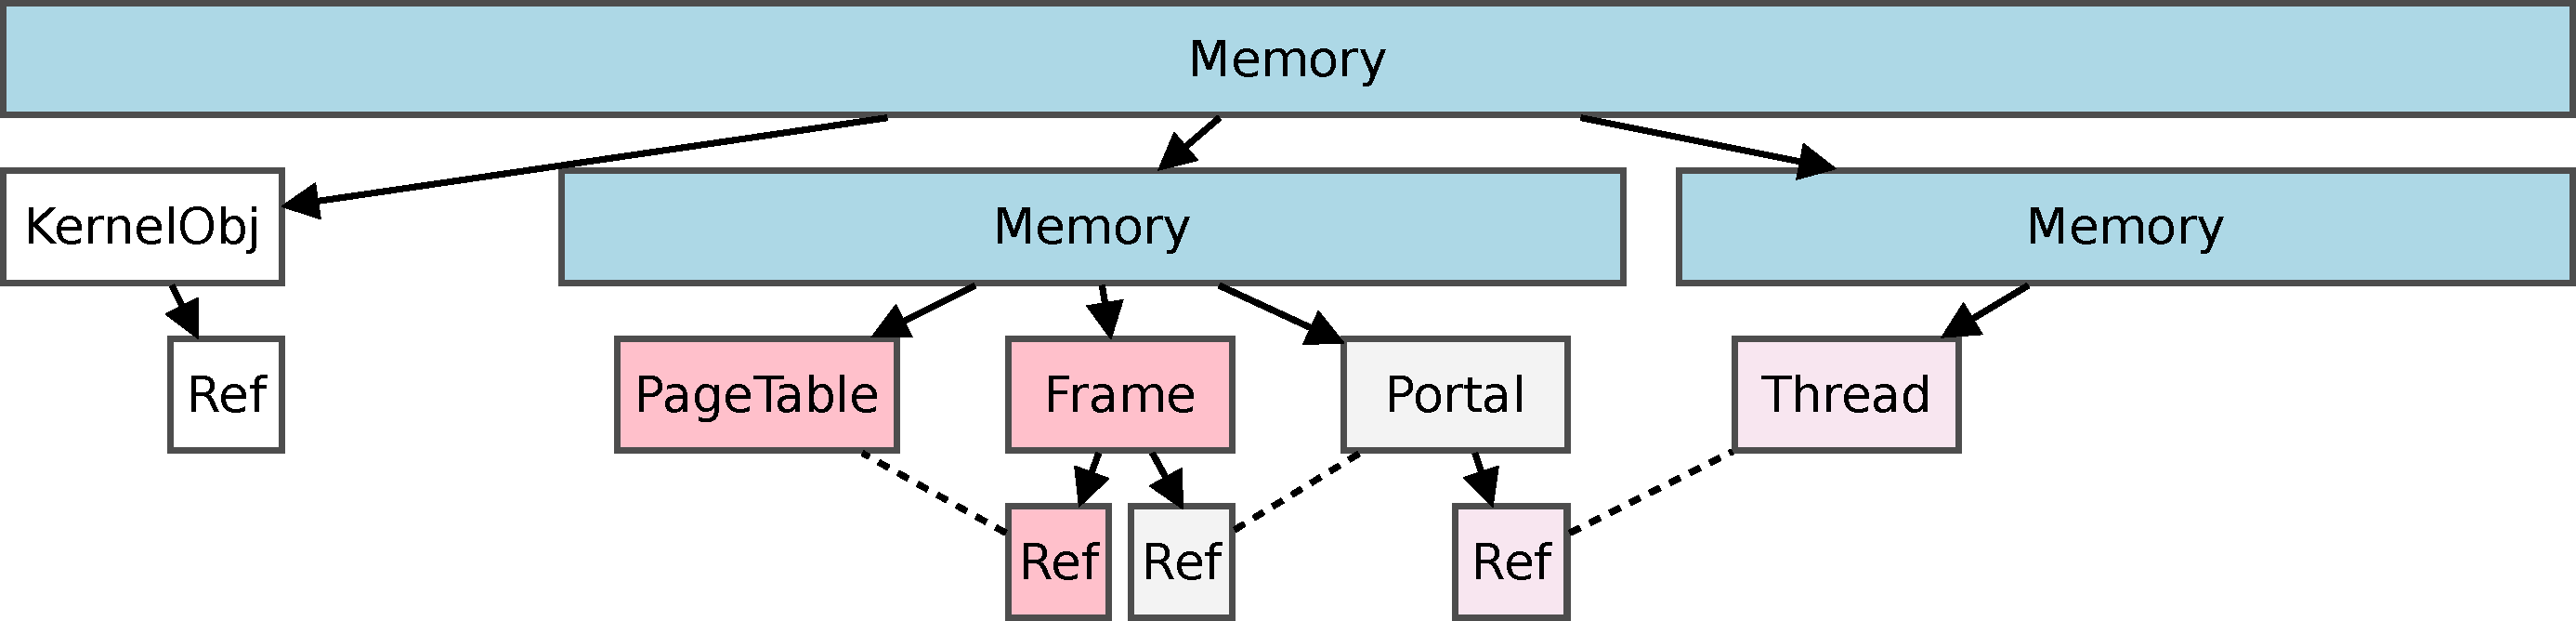
\includegraphics[width=\textwidth]{figures/cap-tree.pdf}
  \end{center}
  \vfill

  \begin{block}{Insight: user-owned pools, explicit allocation}
    \begin{itemize}
    \item allocation via factory system calls; memory provided by application
    \item acyclic resource inheritance: revocable weak references
    \item deferred synchronous deletion
    \end{itemize}
  \end{block}
\end{frame}

\begin{frame}
  \frametitle{System Call Interface}

  \begin{block}{Current state: async.\ RMI imitating C++}
    \begin{itemize}
    \item lookup table: ID $\mapsto$ server stub $\mapsto$  object
    \item access rights via interface inheritance
    \end{itemize}
  \end{block}

  \vfill
  \centering{
    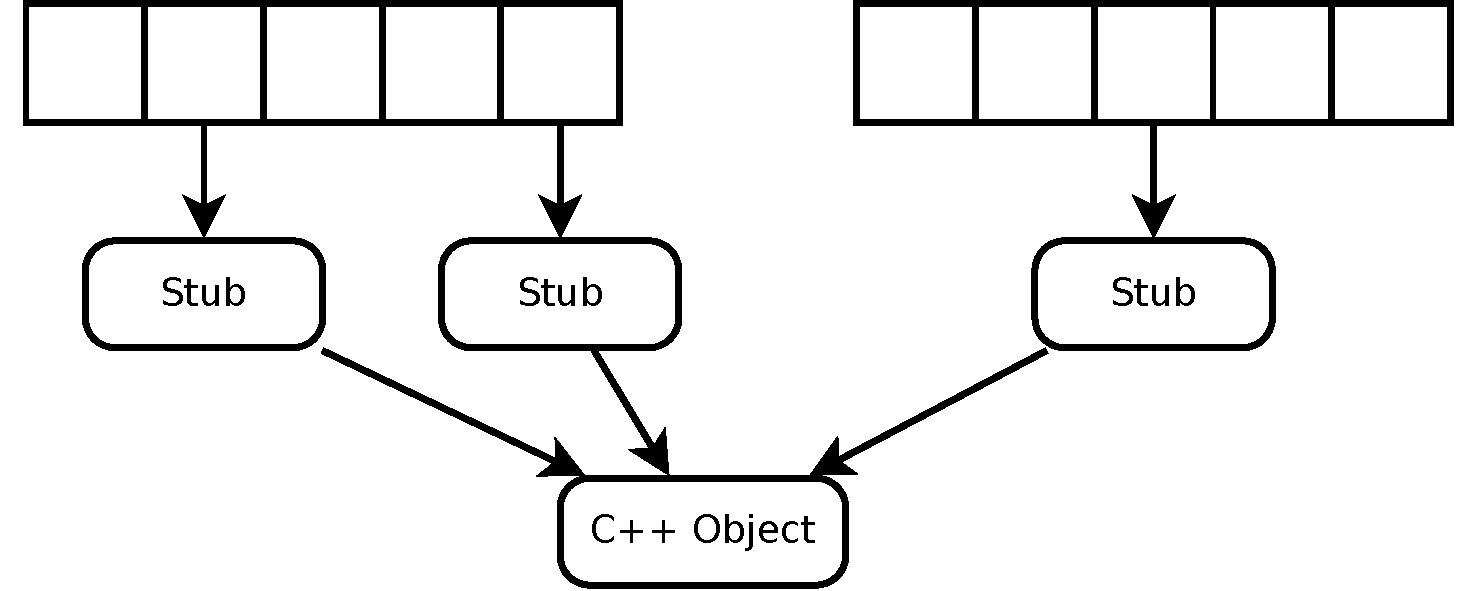
\includegraphics[height=2.5cm]{figures/syscall-stub.pdf}
  }
  \vfill

  \begin{block}{Issues: complex, unreliable}
    \begin{itemize}
    \item resource management: no ownership model, races
    \item access rights: combinatorial explosion of interfaces
    \item transparency \& generated stubs obfuscate call context
    \end{itemize}
  \end{block}
\end{frame}

\begin{frame}
  \frametitle{System Call Interface}

  \centering{
    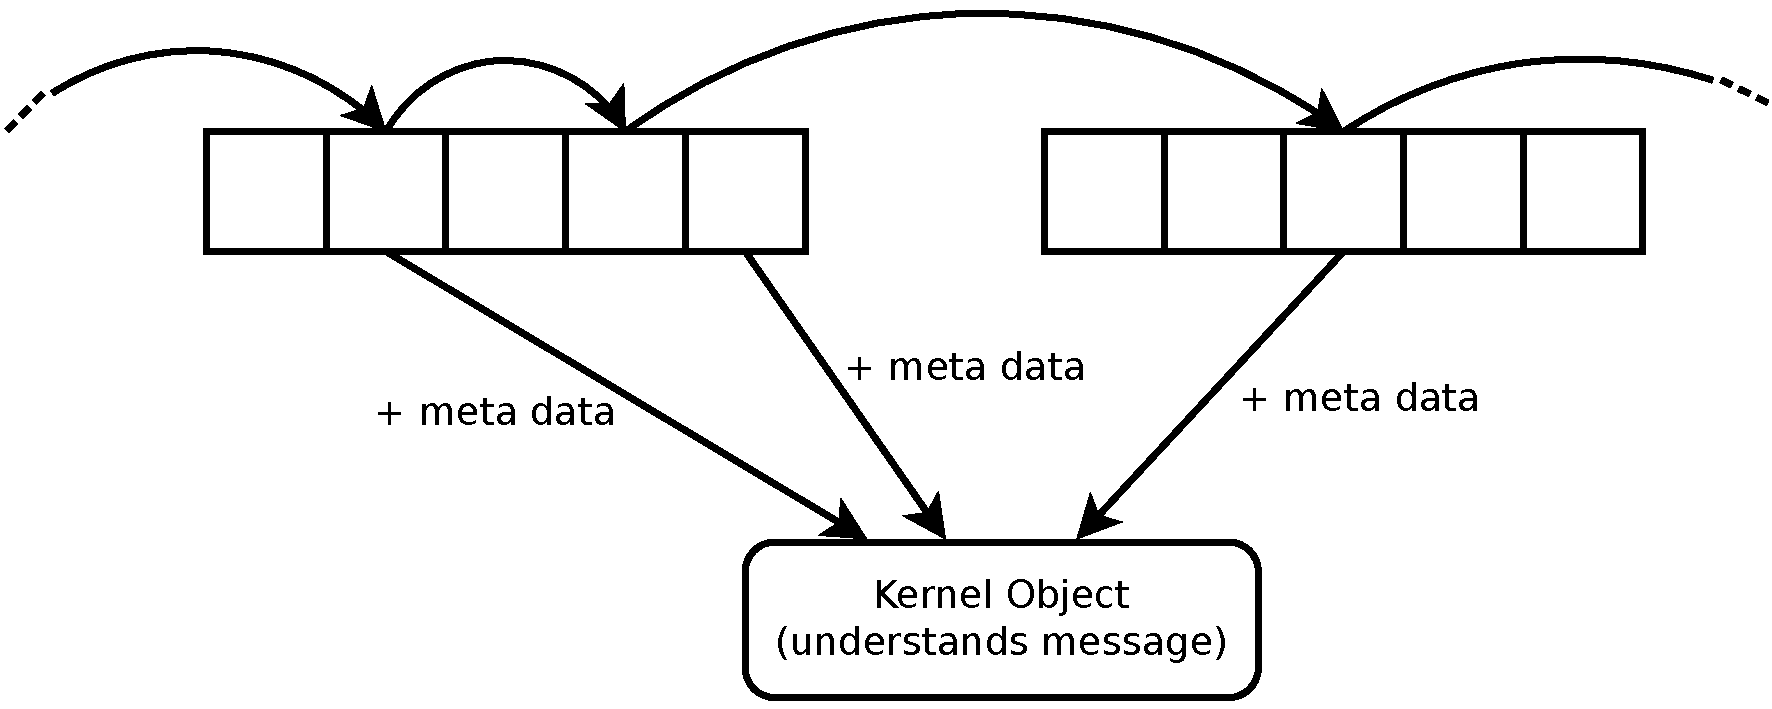
\includegraphics[width=0.6\textwidth]{figures/syscall-kernel-obj.pdf}
  }
  \vfill

  \begin{block}{Insight: build on resource inheritance}
    \begin{itemize}
    \item resource management: tables of weak references
    \item access rights: meta-data in weak references
    \item flow control: deferred synchronous system calls
    \item simplify marshalling
    \end{itemize}
  \end{block}
\end{frame}

\begin{frame}
  \frametitle{Comfort causes Overhead}

  \begin{block}{Issues: kernel policies = comfortable straitjacket}
  \vspace{0.5em}
  \begin{tabular}{lcl}
  one kernel stack per user thread & $\Rightarrow$ & additional allocations\\
  preemptible kernel & $\Rightarrow$ & costly wait-free algorithms\\
  kernel space on logical addresses & $\Rightarrow$ & allocation of page tables\\
  many single-purpose tables & $\Rightarrow$ & coordination overhead\\
  \end{tabular}
  \end{block}

  \vfill
  \begin{center}
  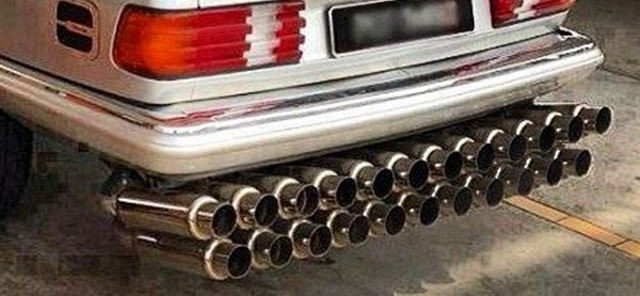
\includegraphics[width=0.4\textwidth]{figures/3-3-a.jpg}
  \end{center}
  \vfill

  \begin{block}{Insight: even a race car is too much}%{Insight: OS as bolts\&pieces -- not race car}
    \begin{itemize}
    \item unify core mechanisms and their interaction
    \item leave distribution and sharing to applications
    \item[$\Rightarrow$] learn more from microkernels\ldots
    \end{itemize}
  \end{block}
\end{frame}

\section{MyThOS Kernel Design 2.0}

\begin{frame}
  \frametitle{Outline}
  \tableofcontents[currentsection]
\end{frame}

\begin{frame}
  \frametitle{Layers based on Communication Model}
  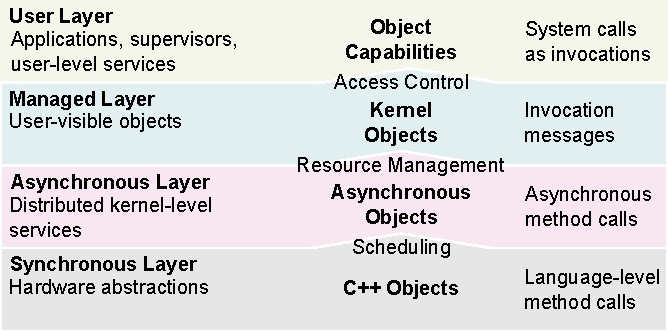
\includegraphics[width=\textwidth]{figures/layers.pdf}
\end{frame}

\begin{frame}
  \frametitle{Asynchronous Objects}
  \framesubtitle{Responsible for mutual exclusion, placement, scheduling}

  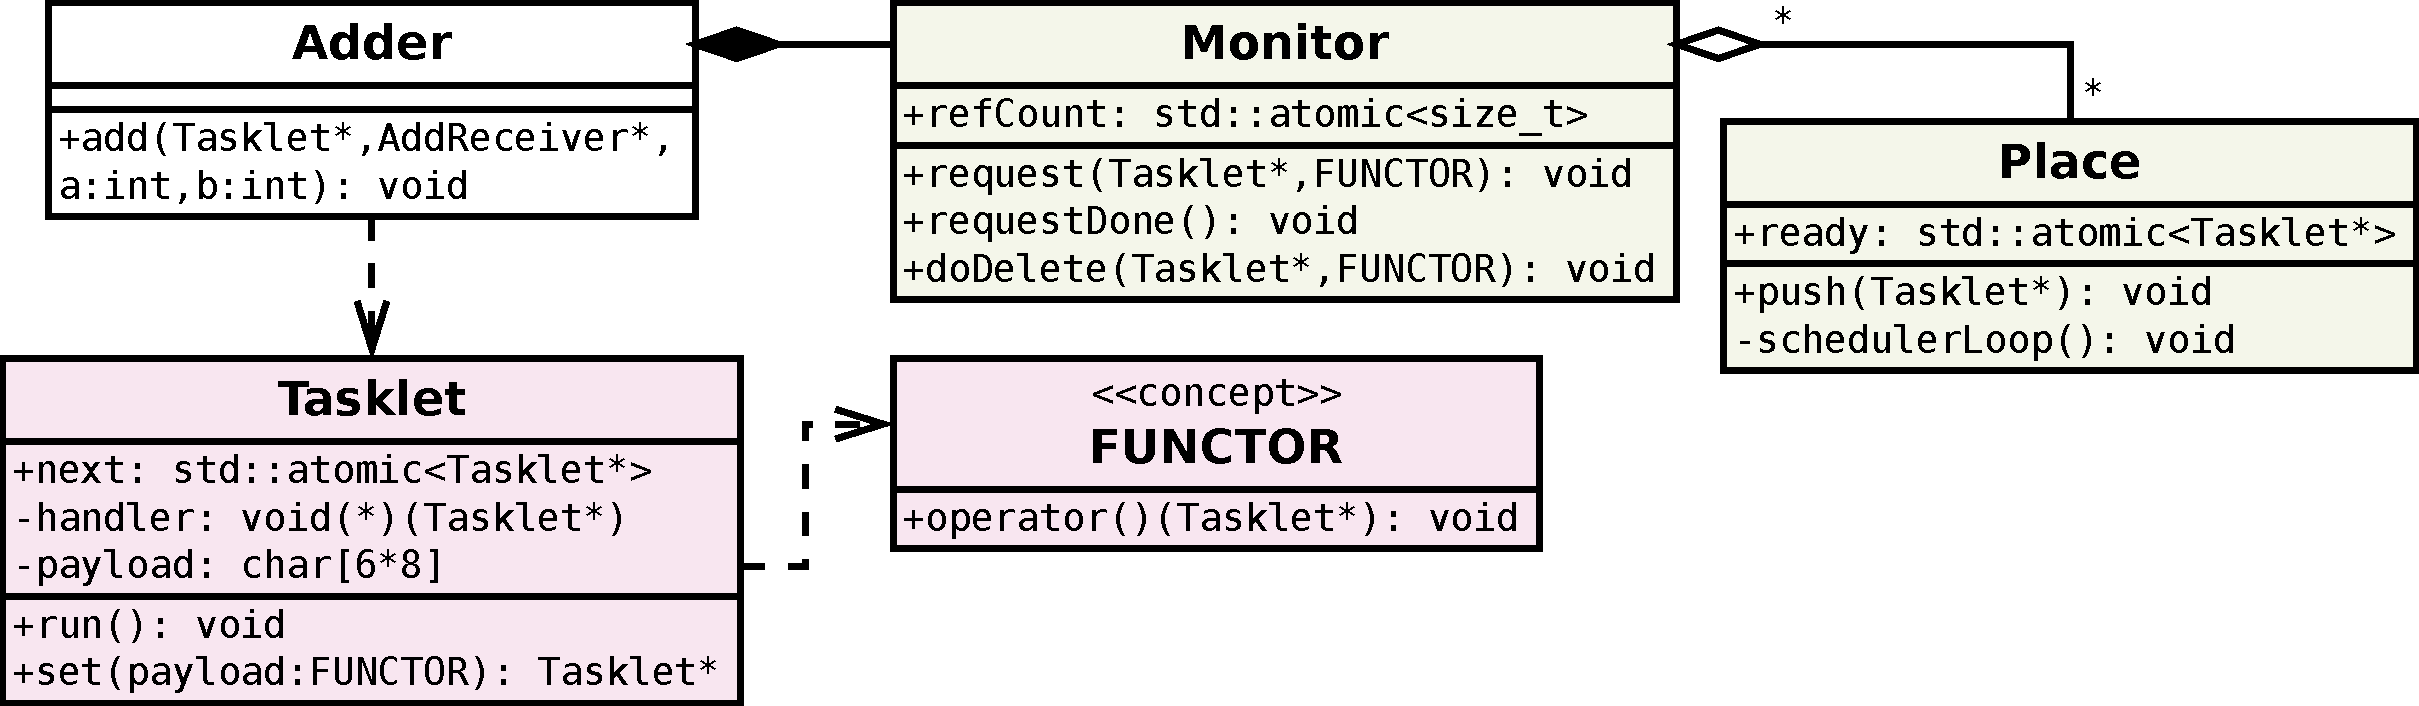
\includegraphics[width=\textwidth]{figures/tasklet-class.pdf}
  \vfill

  \begin{itemize}
  \item tasklet: message buffer, fixed size, statically allocated
  \item flow control: client lends tasklet, response returns it
  \item control flow: server's monitor uses tasklet for scheduling
  \end{itemize}
\end{frame}

\begin{frame}[fragile]
  \frametitle{Asynchronous Objects}
  \framesubtitle<1>{Usage example: Tasklet as flow control credit}
  \framesubtitle<2>{Usage example: C++11 lambda to wrap+unwrap method call}
  \framesubtitle<3>{Usage example: Monitor orders incoming tasks}

  \begin{semiverbatim}
class Adder \{
  \alert<3>{Monitor monitor};
public:
  void add(\alert<1>{Tasklet* t}, AddReceiver* res, int a, int b) \{
    \alert<3>{monitor.request}(\alert<1>{t}, 
            \alert<2>{[=](\alert<1>{Tasklet* t})\{this->addImpl(\alert<1>{t},res,a,b);\}} );
  \}

private:
  \alert<2>{void addImpl}(\alert<1>{Tasklet* t}, AddReceiver* res, int a, int b) \{
    res->result(\alert<1>{t}, a+b);   // do something, then respond
    \alert<3>{monitor.requestDone}();
  \}
\};
  \end{semiverbatim}
\end{frame}

\begin{frame}
  \frametitle{Basic Kernel Objects}
  \framesubtitle{Examples for Kernel Objects}
  \begin{center}
  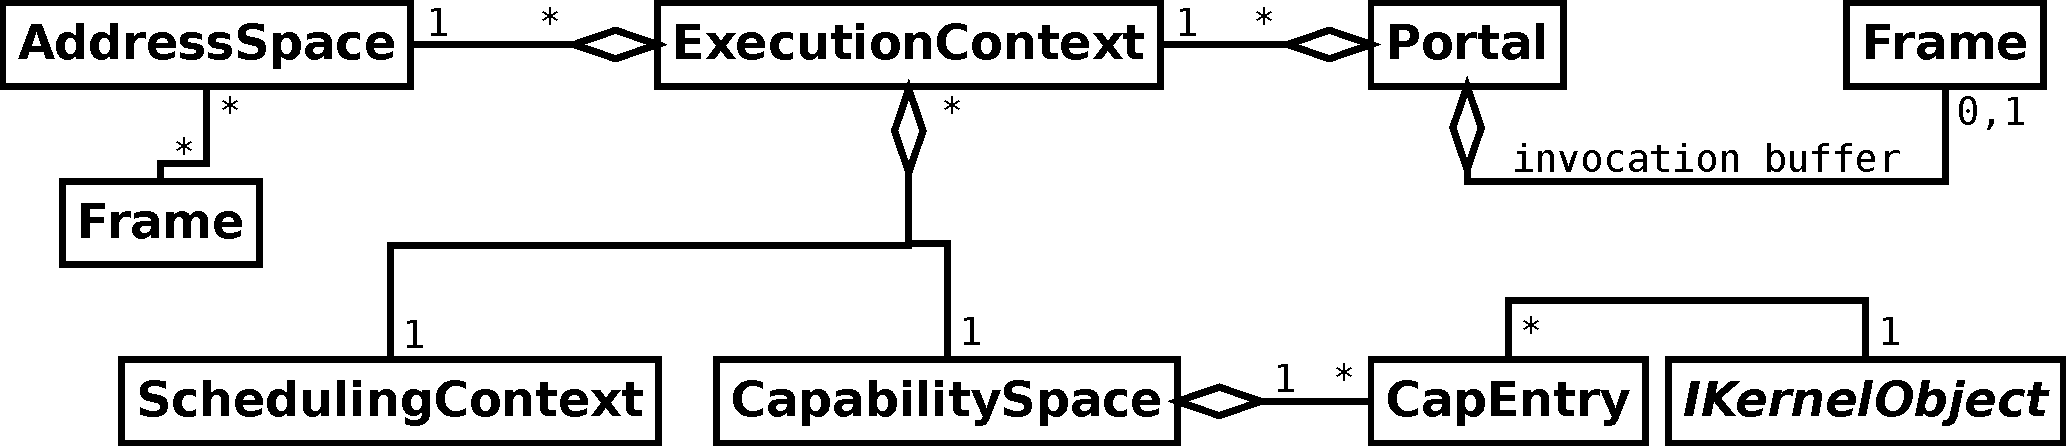
\includegraphics[width=\textwidth]{../fig/kernel-objects-logical.pdf}
  \end{center}
\end{frame}

% \begin{frame}
%   \frametitle{Kernel Heap}
%   \framesubtitle{Where do all these Kernel Objects come from?}
%   \begin{block}{Issues}
%     \begin{itemize}
%       \item generous use of the Kernel Heap %(low-level)
%       \item balancing needs communication %(high-level)
%       \item communication may needs additional memory %(low-level)
%     \end{itemize}
%   \end{block}
%   \begin{block}{More trouble}
%     \begin{itemize}
%       \item \emph{locality:} local vs. remote vs. global heaps
%       \item \emph{sharing:} private vs. shared heaps
%       \item \emph{control:} limit and revoke access to kernel memory
%     \end{itemize}
%   \end{block}
% \end{frame}

\begin{frame}
  \frametitle{Untyped Memory}
  \framesubtitle{Where do all these Kernel Objects come from?}
  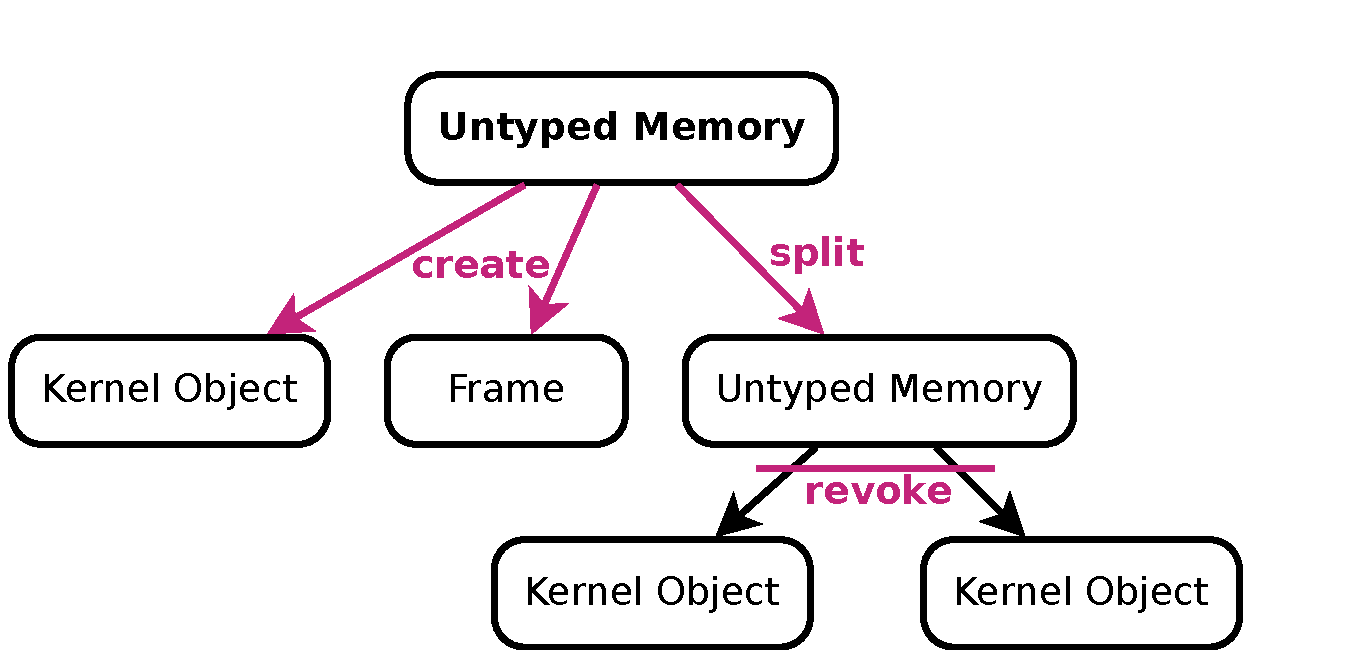
\includegraphics[width=\textwidth]{figures/um-ops.pdf}
\end{frame}


\begin{frame}
  \frametitle{Resource Inheritance}
  \framesubtitle{Inheritance tracking through Capabilities}
  \begin{center}
  % chose one
  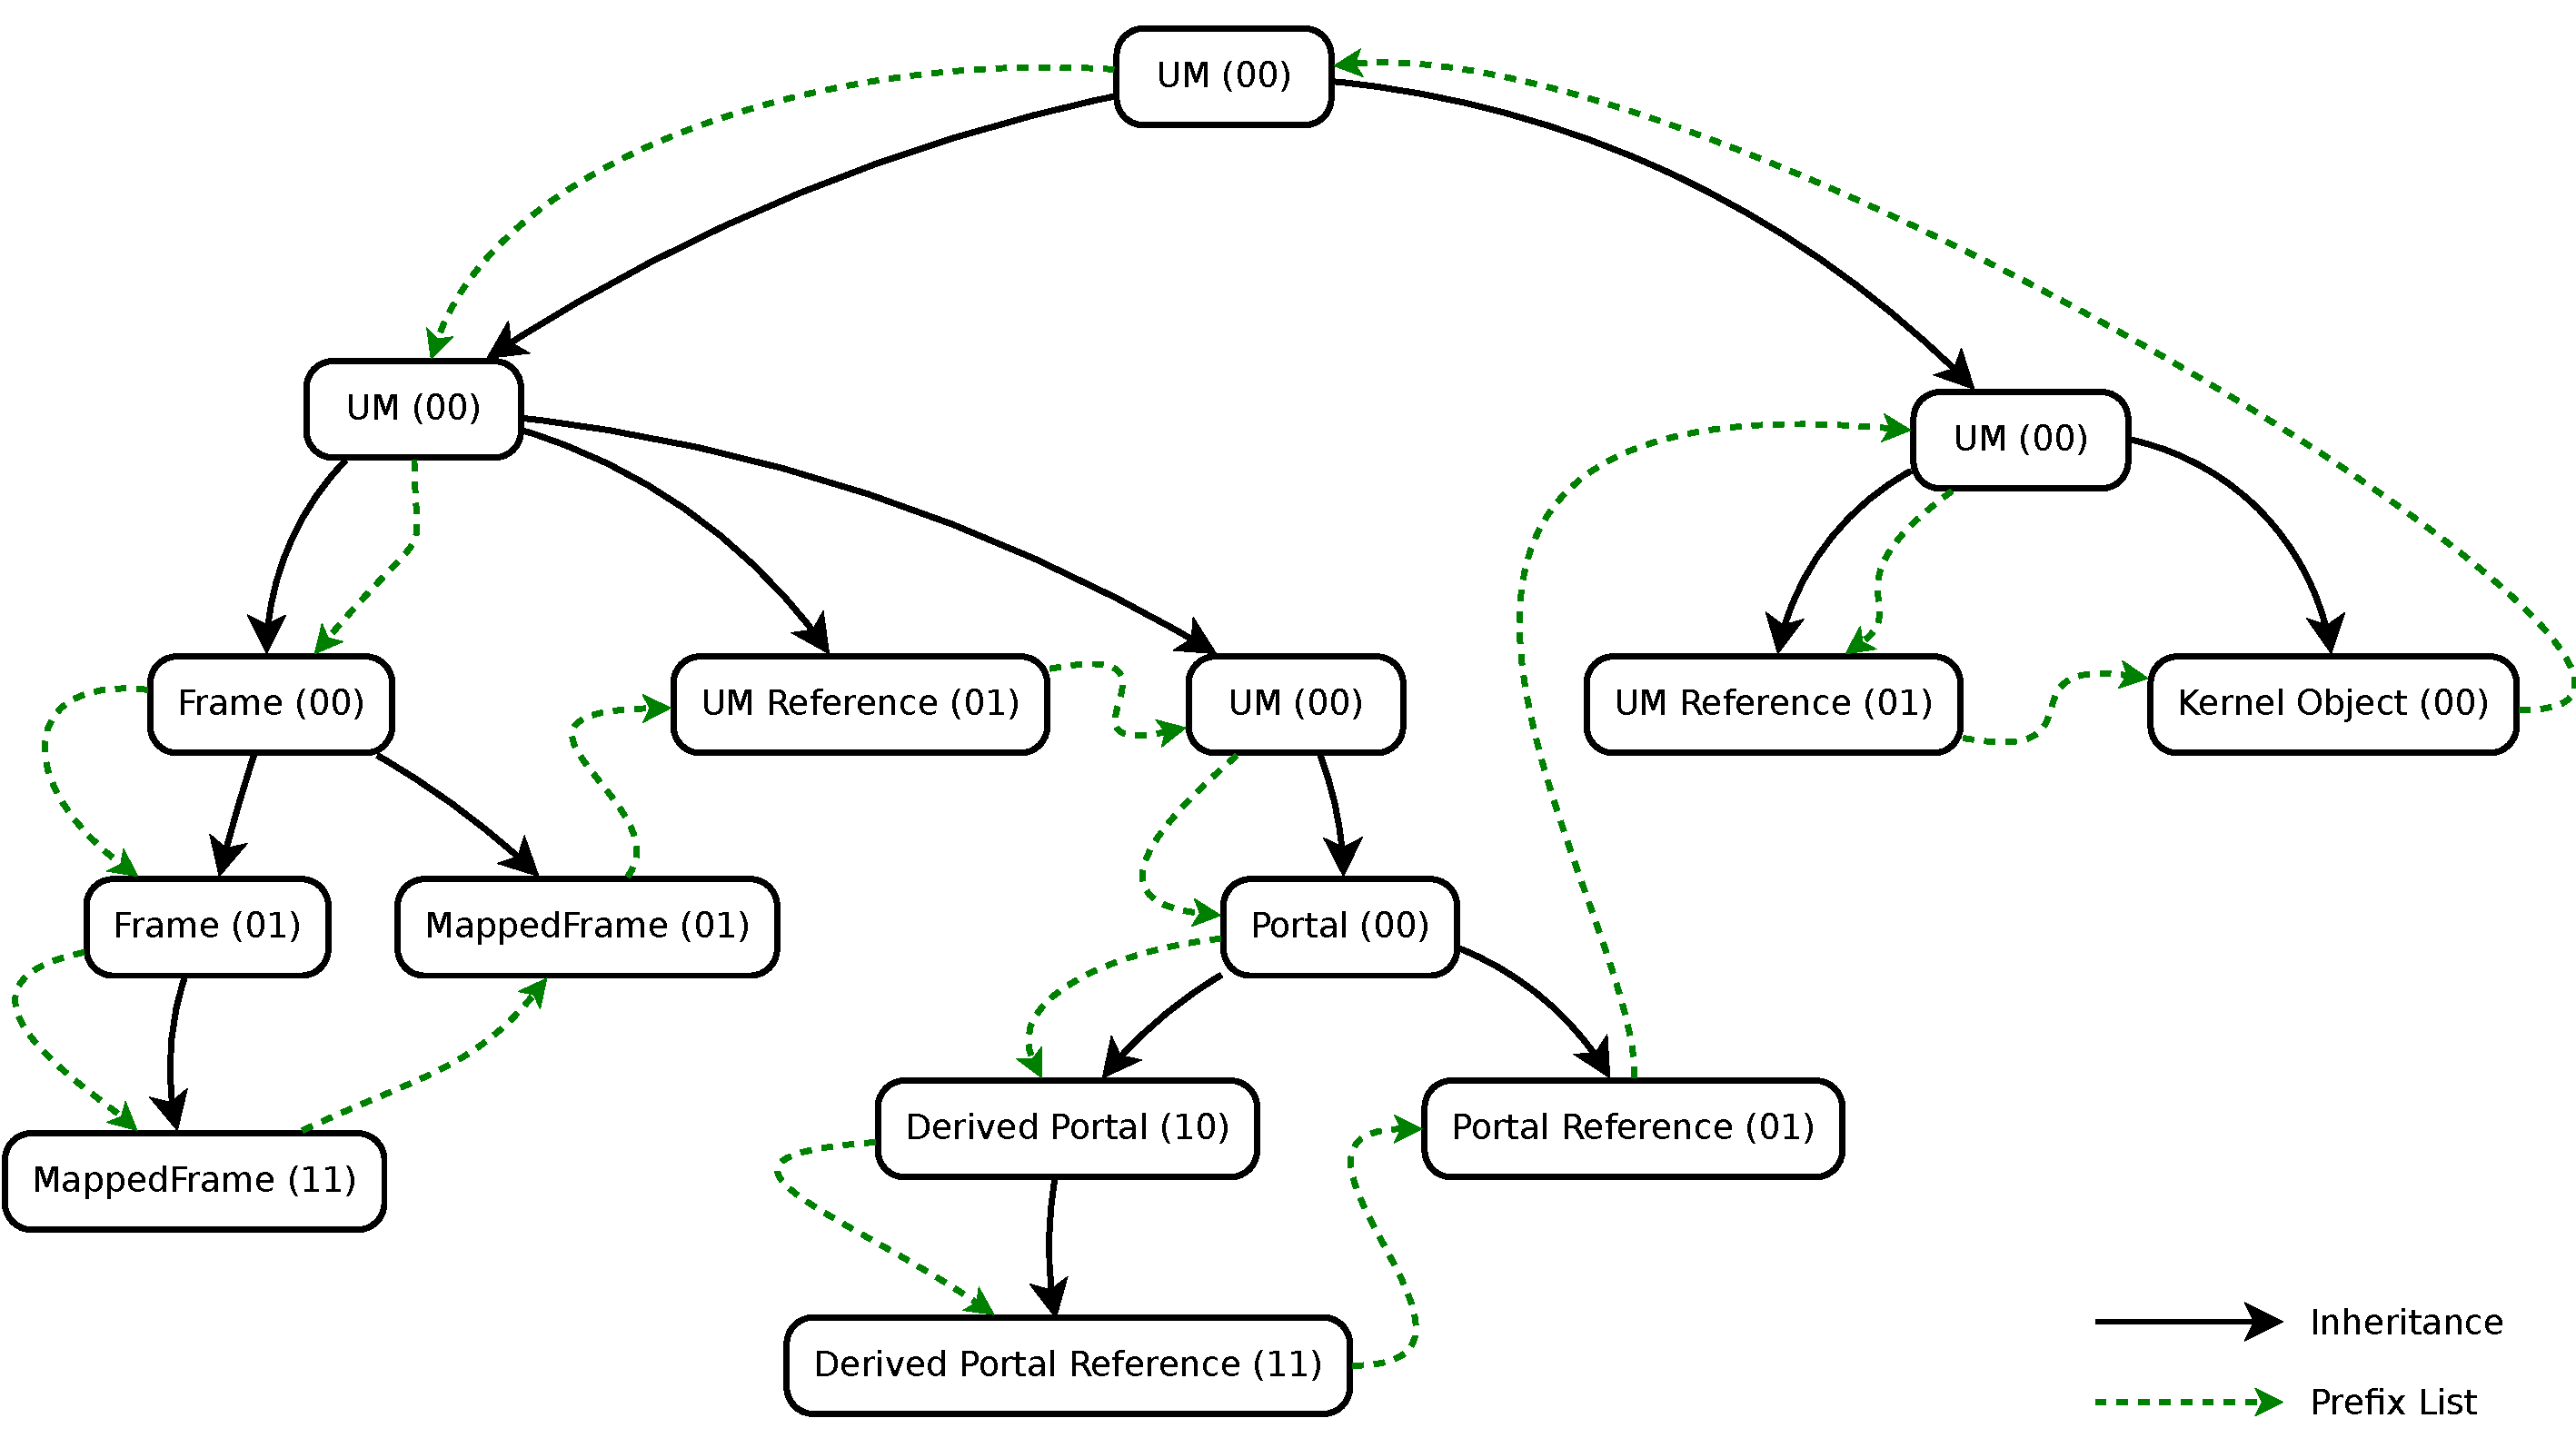
\includegraphics[width=\textwidth]{../fig/cap-tree.pdf}
  %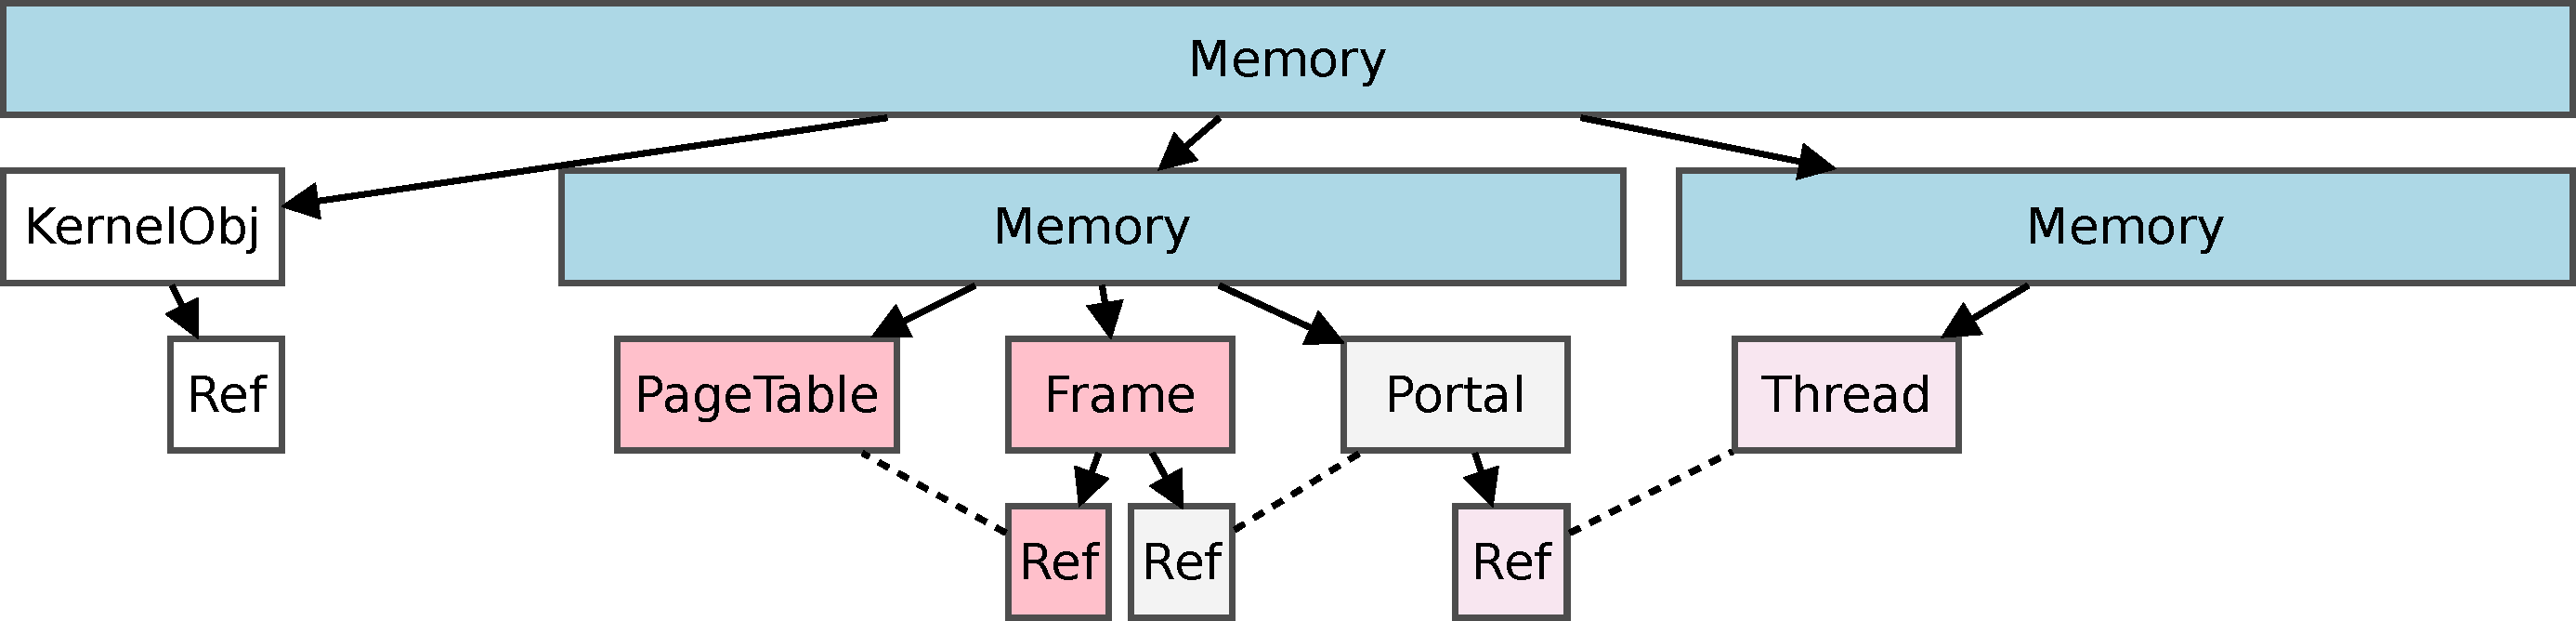
\includegraphics[width=\textwidth]{figures/cap-tree.pdf}
  \end{center}
\end{frame}

\begin{frame}
  \frametitle{Capability types}
  \framesubtitle{Derived and Reference Capabilities}
  \begin{center}
  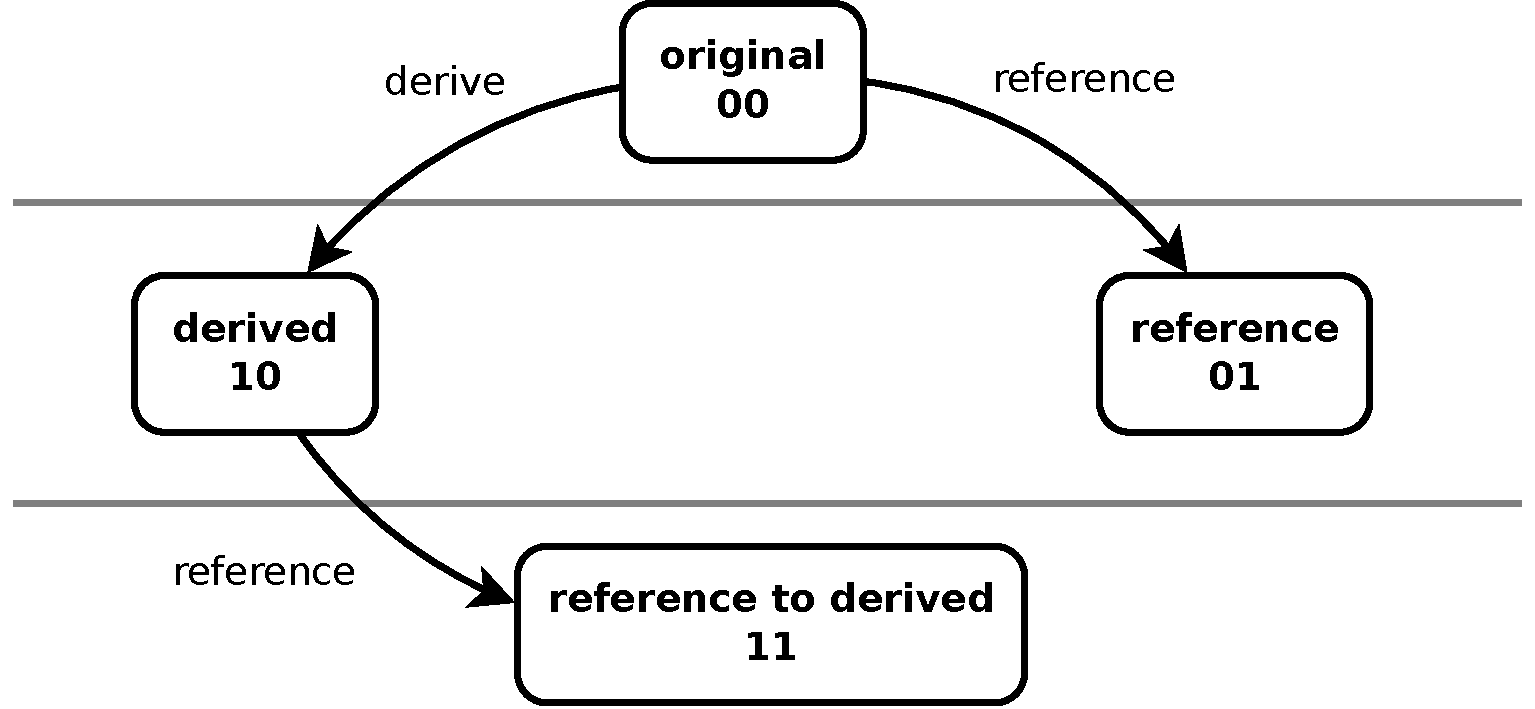
\includegraphics[width=0.75\textwidth]{../fig/DerivedReferenceBits.pdf}
  \end{center}
\end{frame}

\begin{frame}[fragile]
  \frametitle{Object Invocation: Kernel Side Dispatcher}

    \begin{semiverbatim}
void Adder::invoke(Tasklet* t, Portal* ctx, CapEntry* cap) \{
  switch (ctx->protocol()) \{
  
  case ADDERPROT:
    switch (ctx->method()) \{
    
    case ADD: 
      \alert{monitor.request(t, [=](Tasklet*t)\{this->add(t,ctx,cap);\} );}
      return;
    \}
    break;
  \}
  ctx->response(t, CORE, UNKNOWN_METHOD);
\}\end{semiverbatim}

\end{frame}

\begin{frame}[fragile]
  \frametitle{Object Invocation: Kernel Side Method}
    \begin{semiverbatim}
void Adder::add(Tasklet* t, Portal* ctx, CapEntry* cap) \{
  int a, b;
  bool success = \alert{ctx->readMsg(a,b);}

  if (\alert{AdderCap(cap).canAdd()}) \{ 

    // work with ctx->thread(), cap, a, b ...
    \alert{ctx->response(t, ADDERPROT, SUM, a+b);}

  \} else ctx->response(t, CORE, DENIED); 
  monitor.requestDone();
\}\end{semiverbatim}
\end{frame}


\section*{Conclusions}

\begin{frame}
\frametitle{Thanks for listening}
\begin{block}{Progress}
\begin{itemize}
\item streamlined asynchronous programming model
\item eliminated all on-demand allocation
\item application decides on sharing and distribution
\item unified resource management and deallocation
\item simplified client/server stubs for object invocation
\end{itemize}
\end{block}
\end{frame}

%\begin{frame}
%\frametitle{Literatur}
%\bibliographystyle{alphadin}
%\bibliography{../literature}
%\end{frame}

\appendix

\begin{frame}
  \frametitle{Concurrent Object Deallocation}

  \begin{enumerate}
  \item mark root reference as zombie
  \item recursively revoke all children in inheritance tree:
  \item[$\Rightarrow$] informs reference holders, ack.\ as continuation
  \item broadcast task to all active cores
  \item[$\Rightarrow$] safeguard against temporary references
  \item call async.\ deletion method of the object
  \item[$\Rightarrow$] delayed by monitor until all pending tasks done,\\
    return memory to parent, ack.\ as continuation
  \item respond via ack.\ continuation
  \end{enumerate}
\end{frame}

\begin{frame}[fragile]
  \frametitle{Object Invocation: User Side Proxy Pointer}

    \begin{semiverbatim}
void Adder::add(Portal* p, Future f, int , int b) \{
  p->invoke(this->obj, ADDERPROT, ADD, f, a, b); 
\}

// \ldots in app's idle loop:
Portal* res = wait();
if (res) res->handleResponse(); // pushes results to f
    \end{semiverbatim}  

  \begin{itemize}
  \item \texttt{p} same role as tasklets, larger message
  \item \texttt{Future f} depends on user's programming model
  \item based on C++11 variadic templates and \texttt{operator<<}
  \end{itemize}
\end{frame}

\begin{frame}
  \frametitle{Many Threads Operating System}
  %\framesubtitle{}

  \begin{center}
    
\includegraphics[scale=0.3]{mythos-logo}
  \end{center}
  \vspace{0.5cm}

  \begin{itemize}
  \item[\textbf{Ziel}] \alert{dynamische} HPC Anwendungen auf \alert{Vielkern-Prozessoren}
  \item[\textbf{Fokus}] schnelle Thread-Verwaltung
  \item durchschnittlicher Durchsatz statt worst-case Latenz
  \item BMBF Projekt\footnote{Fördernummer BMBF 01IH13003} von Uni Ulm, mit Uni Siegen, BTU Cottbus, \\ Alcatel-Lucent Deutschland AG, HLRS Stuttgart
  \end{itemize}
\end{frame}

\begin{frame}
  \frametitle{Multi- versus Many-Core}

  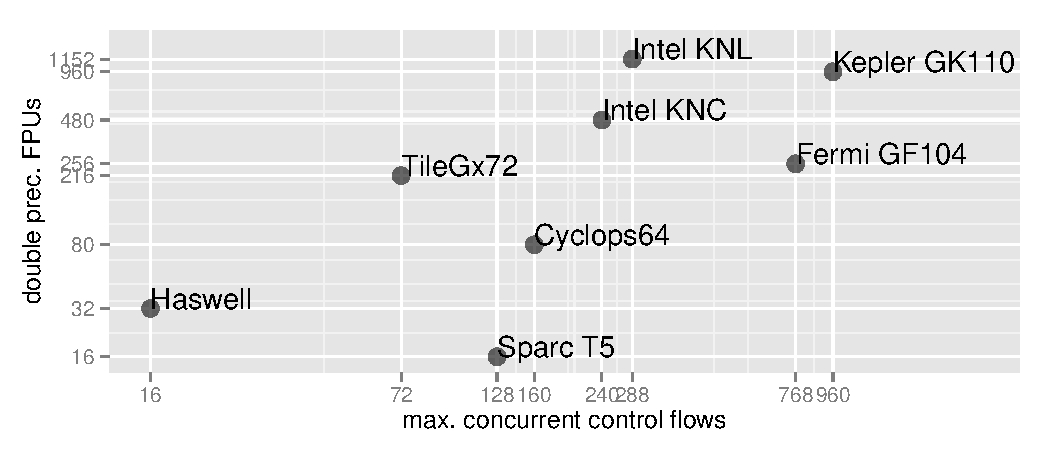
\includegraphics[height=5cm]{figures/manycore}

  \begin{itemize}
  \item max. paralleler Durchsatz in geg. Power- \& Platz-Budget 
  \item Energie- \& Platzeffizienz statt Single-Thread Performance 
  \item[$\Rightarrow$] \alert{Durchsatz nur durch Aufgaben- und Daten-Parallelität }
  \end{itemize}
\end{frame}

\begin{frame}
  \frametitle{Zielarchitektur: Intel XeonPhi KNC}
  %\framesubtitle{Intel Xeon Phi Knights Corner}

  \begin{center}
    %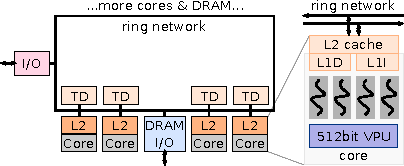
\includegraphics[height=2cm]{figures/hw-xeonphi}
    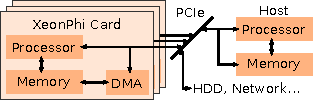
\includegraphics[height=2cm]{figures/hw-xeonphi-host}
  \end{center}

  \begin{itemize}
  \item 60 Kerne: In-Order, keine Sprungvorhersage, 2 Takte Instruction Decode
    % consequence: low single-thread performance, sensitive to branches
  \item 4 HW Threads per Core: gemeinsamer L1+L2 Cache,\\ 
    gemeinsamer TLB, keine Global Pages, keine TLB PCIDs 
    % consequence: switching between address spaces is expensive
  \item 8GiB Hauptspeicher: $<$35 MiB per Thread,\\
    Cohency Latenz $>$200 Takte, pseudo-uniform, kein MWAIT
    % consequence: cannot be used like pure distributed memory system, synchronisation and communication via shared memory curbed by slow CC  
  \item PCIe Karten: unterstützen custom OS Kernel,\\
    Kommunikation mit Host über gem. Speicher
    % consequence: easy to experiment with
  \item[$\Rightarrow$] \alert{Ideale Worst-Case Plattform!?}
  \end{itemize}
\end{frame}

\begin{frame}
  \frametitle{Szenario I: HPC Simulationen}
  \framesubtitle{Moleküldynamik (HLRS), Strömungen und Elektrodynamik (Uni Siegen)}

  \begin{itemize}
  \item eine Anwendung besitzt ``alle'' Kerne und Speicher
  \item Aufgabenverwaltung und Kommunikation auf Anwendungsebene
  \item dynamische Speicherverwaltung
  \end{itemize}

  \begin{block}{Anforderungen}
    \begin{itemize}
    \item effizientes Warten statt Polling (min Energie, min Contention)\\
      Semaphore/Futex \texttt{wait}, \texttt{signal}
    \item viele Threads manipulieren gemeinsamen Adressraum (IO,PGAS,DSM)\\
      \texttt{mmap}, \texttt{mremap}, \texttt{mprotect}
    \end{itemize}
  \end{block}
\end{frame}

\begin{frame}
  \frametitle{Szenario II: Compute Cloud}
  \framesubtitle{Verteilte Medienverarbeitung (Alcatel/CenoLabs)}

  \begin{itemize}
  \item dynamisch konfigurierter Datenfluss-Graph
  \item Knoten aktiviert durch Input Daten, laufen in Isolation+Zeitschranke
  \item Cloud Manager bewegt Daten, migriert Knoten für min. Energie
  \end{itemize}

  \begin{block}{Anforderungen}
    \begin{itemize}
    \item viele Threads mit eigenem Adressraum erzeugen und aktivieren\\
      \texttt{create}, \texttt{destroy}, \texttt{activate} mit Zeitschranke
    \item Manager manipuliert fremde Adressräume, z.B. zero-copy comm\\
      \texttt{mmap}, \texttt{mremap}, \texttt{mprotect} auf Kind-Threads
    \item Weiterleiten der Systemaufrufe, Exceptions etc. an Manager\\
      \texttt{event queue}
    \end{itemize}
  \end{block}
\end{frame}




\end{document}
